\chapter{Methods}
\label{chap:method}

This chapter will cover the specific implementation details of the concepts researched in this thesis. To reiterate, this work conducts a systematic investigation on performance of previous state 
of the art IAD approaches on logical anonomalies and interprets the results. Secondly this paper introduces a feature level ensemble approach for combining potentially heterogeneous anomaly detection methods to achieve greater robustness. 
The just named contributions 
are thematized in regards to their execution in the respective sections \ref{sec:lcocsurveymethods} and \ref{sec:ourensemblenetwork} of this chapter.


\section{Logical Anomaly Detection}
\label{sec:lcocsurveymethods}

As discussed in the introductory chhapter \ref{chap:introduction}, logical anomalies represent a signifacant part of image anomaly detection in modern
manufacturing settings. The experiments also serve as an extensive comparison of SOTA methods for IAD versus recent approches that where 
introduced with special mind to logical anomalies, like GCAD \cite{LOCODentsAndScratchesBergmann2022}. 
Moreover, for a qualitative evaluation of the performance change when using feature level ensembles, one first needs to evaluate the base performance 
of each relevant classifier of the set. 
Hence this work features experiments to evaluate IAD approaches mainly evaluated on the classical MVTecAD dataset. To do so, the original 
code from each paper was taken and not modified in regards to any reportet parameters and/or arguments. This was to prevent possible unwanted deviations 
in original performance by changing up synergies of hyperparameters. This paper recognizes the possibility of improved performances on the logical anomalies dataset 
with different combinations of model parameters. Yet this work focusses on the result assessment of current unmodified apporoaches and 
more importantly the increased robustness through the use of ensembles. Therefore research regarding this hypothetical improvement would 
have to be done in a future work. Metrics that are specifically looked at in this context are the AUROC, pixel AUROC(weitere maybe einfpgen) and the sPRO. 
If the functionality to evaluate these metrics was already given, the results of inference were taken from the original code, else the according functionality 
was implemented in this work and used to produce the according metrics. Moreover the results investigate possible causes and effects regarding the segmentation/localization results of the 
classifiers. This is not done according to an official metric but in a more descriptive sense.
Papers whose approaches were evaluated using the MVTecAD LOCO dataset were: SimpleNet \cite{liu2023simplenet}, PatchCore \cite{patchCore2022}, \cite{csflow2022} and \cite{Zavrtanik_2021DRAEM}. (list of paper references with names). 
These papers were discussed in more depth in the backgrounds section and any specifics like 
hyperparameters can be viewed in the corresponding paper. Furthermore all named classifiers were including, among other variable measures, 
a preprocessing step to resize the input image. This makes for a variable model input and also the ability to process rectangular images, 
which is important due to MVTecAD LOCO images being rectangular unlike the squared input from the standard MVTecAD dataset. The only 
necessary modification to the whole process of anomaly detection was the generation of image masks. The MVTecAD LOCO dataset stores its 
masks in multiple seperate black and white images, one for each individual anomaly. To fix errors stemming from this fact, additional 
code was added that pastes all masks belonging to one image into a single mask before iterating through the data. 
%nachfolgender satz drinnen lassen?
There also exists a minor ablation experiment experimenting with the elimination 
of possible background artifact removal on images of our novel dataset category. For this we programmatically set every pixel in a certain radius around the main object to black, to investigate 
segmentation artifacts of certain classifier methods. The results can be viewed in section xyz.




\section{Ensemble network}
\label{sec:ourensemblenetwork}

!BILD von pipeline machen!

!abändern!
- schreiben dass wir hier verschiedene feature representations leveragen wollen

The following subsections deal with the individual components of our ensemble network pipeline, referencing concepts discussed in chapter \ref{chap:background}. This network is conceptually based on 
different approaches. First we produce cut off models and an ensembling mechanism in accord to \cite{EnsembleHeller2023}. For the actual IAD process, this approach is based on the SimpleNet method \cite{liu2023simplenet}. 
The discriminator presented there potentially makes for an easy to implement, yet powerfull method of differentiating between anomalous and normal images, as seen by the performance of the original 
SimpleNet approach. 


\subsection{Ensemble Members}
\label{sec:ensemblecandidates}

For the ensemble to be one, we need different feature representations to combine. Since the overall ensemble strategy heavily relies on SimpleNets \cite{liu2023simplenet} architecture 
it is fitting to utilize different simplenet backbones for an exploratory approach. For this we chose three different pretrained backbones. Each one was from one of the three 
model structures: Wideresnet \cite{wideresnet}, VGG \cite{VGG} and VIT \cite{VIT}. 

- schreiben welche backbones specifically und performance kurz ansprechen und erklären.

One aspect to keep in mind is that the backbones are pretrained and do not necessarily have feature outputs in the same latent space % stimmt die aussage?
and may also not produce inherently useful ones. To bridge this problem we trained a feature adapter from SimpleNet for each of the backbones, before ensembling the features. 
This ensures that all feature representations are in the same space and can be properly ensembled. The resulting feature vectors are also projectred with an additional global 
feature adapter

- schreiben dass wir auch wideresnet50 nehmen mit verschiedenen hierarchies weil wir uns dadurch erhoffen die verschiedenen levels an feature representations zu leveragen

\begin{figure}[htbp]
    \captionsetup[subfigure]{justification=centering}
    \centering
    \begin{subfigure}[b]{0.25\textwidth} % Decreased width to add space
        \centering
        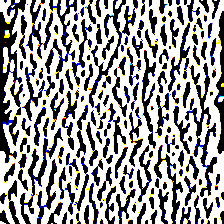
\includegraphics[width=\textwidth]{figures/featurelayersviz/low_channel.png}
        \caption{Lower Level Features}
    \end{subfigure}
    \hspace{0.05\textwidth} % Add space between subfigures
    \begin{subfigure}[b]{0.25\textwidth} % Decreased width to add space
        \centering
        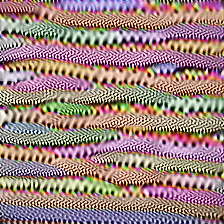
\includegraphics[width=\textwidth]{figures/featurelayersviz/medium_channel.png}
        \caption{Mid Level Features}
    \end{subfigure}
    \hspace{0.05\textwidth} % Add space between subfigures
    \begin{subfigure}[b]{0.25\textwidth} % Decreased width to add space
        \centering
        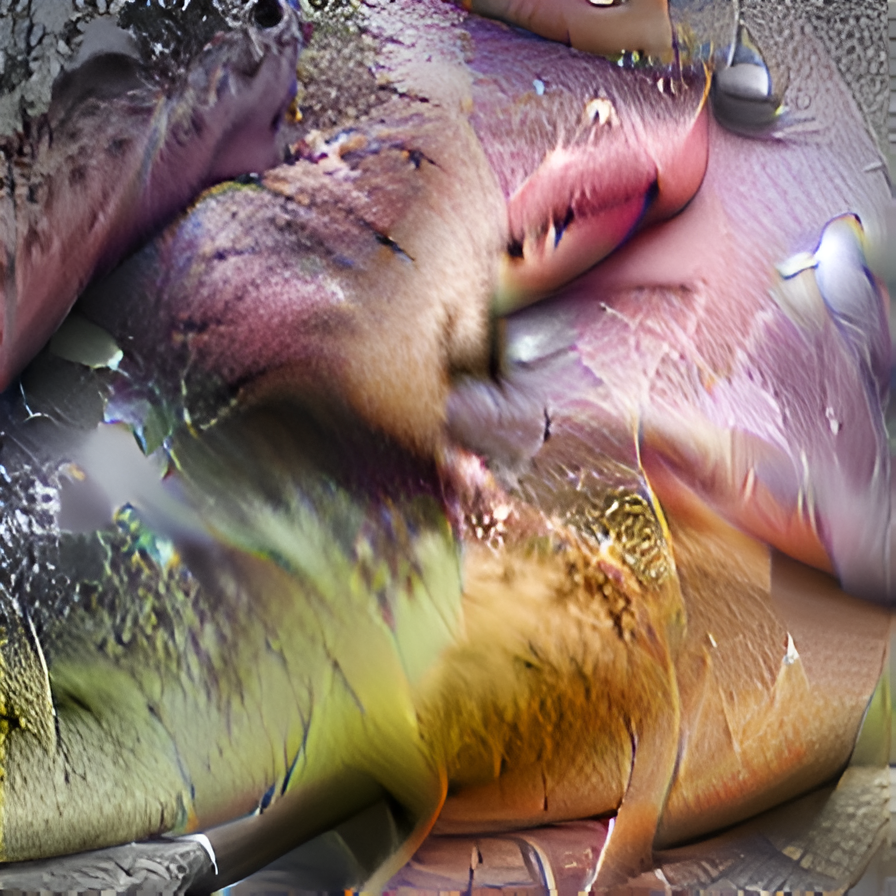
\includegraphics[width=\textwidth]{figures/featurelayersviz/late_channel.png}
        \caption{Higher Level Features}
    \end{subfigure}
    \caption{Illustration of Feature Representations at Different Levels}
    \label{fig:featurelayers}
\end{figure}


!unten neu schreiben!


The first exploration of the ensemble method is done with the IAD methods PatchCore \cite{patchCore2022} and SimpleNet \cite{liu2023simplenet} as ensemble members. These two 
are conveniently both creating features in form of locally aware patches, making for easy preprocessing before ensembling. For combining them on a 
feature level, we need to intersect the trained models somewhere during the inference process to then exctract accurate representations that can be used. 
For SimpleNet this cut-off is happening after the extracted features are projected through the trained feature adapter (the green tiled pane in figure xyz). 
PatchCore requires more work, as the feature extraction and patch converting steps are essentially the same to the ones in SimpleNet. Moreover there are no alterings of resulting feature vectors 
after these steps, only nearest neighbor search. Yet solely utilizing features extracted 
from the pretrained feature extractor would not be sensible, since it would not add any new information to the ensemble that was not already represented in SimpleNets patch vectors. 
The approach realized in this work is based on the way patchcore scores its image anomalies. Since its decisions are fundamentally based on the L2 norm of the difference between newly extracted 
features and the nearest feature vector in the memory bank (see equation \ref{eq:patchcoredistance}), it is to be assumed that there is information in the differences of the vectors. Thus the 
feature representation $m^{final}_i$ for a image patch $p_i$ is derived as $m^{final}_i = | m_i^{test} - m |$ where $m \in \mathcal{M}$ with $\mathcal{M}$ as the memory bank, $m_i^{test}$ as the 
according input patch vector and $m$ as the neirest neighbor of $m_i^{test}$. Additionally we introduce a projection layer similar to \cite{liu2023simplenet} which is supposed to help project the 
features taken from this ensemble member to be in a similar space as the ones by SimpleNet, which are already projected from the start. The nature of this projection layer is again a single 
layer network, being applied to the difference vectors.



\subsection{Feature Level Ensembling}
\label{sec:featurelevelensemble}

For combining the feature representations from different ensemble members, we chose the approach of the independent transformation block (see figure \ref{fig:ITBheller}, section \ref{sec:ensembles}). This means 
PCA was first performed on each set of feature vectors, before then resizing and concatenating them. The PCA was performed via the scipy library and fitted on the training data. As for resizing, 
the feature vectors were bilinearly interpolated to the largest diimensions of the ensemble candidates. Moreover the amount of feature maps kept per classifier, namely $\alpha$ in figure \ref{fig:ITBheller}, 
was derived by dividing up the number of feature maps from the first classifier in the list of ensemble members, which in this instance also was the maximum amount. If the number 
was not evenly divisible, excess maps would be split up among the remaining classifiers as evenly as possible.\newline
As stated in the results under subsection \ref{subsec:ITBfail} and further analysed in section \ref{subsec:ITBfailconc}, this approach did not yield the expected results. 
A solution to shortly bridge this problem was to simply stack the channels of the ensemble members feature maps. This produced the results shown and discussed in respective 
sections \ref{subsec:stacking} and \ref{subsec:stackingconc}.


\subsection{Ensemble Training}
\label{sec:discriminator}
Our approach to use a small, compact discriminator to differentiate between regular and anomalous image features is based on the concept of 
the one-class classification class from the representation based approaches. Specifically the main inspiration of this work is the approach 
presented in SimpleNet \cite{liu2023simplenet}. Since our discriminators inputs in the ensemble pipeline, which stems from ensembled locally aware patch features, 
will be of the same nature as 
the inputs for SimpleNet's discriminator, it is reasonable to utilize their network architeture for this work. Looking back at section 
\ref{subsec:simplenet} and moreso figure \ref{fig:simplenetpipeline}, we thus will adapt the SimpleNet pipeline at the feature adapter step. 
This means, we will train a global feature adapter that ensures the projection of ensembled features into the right latent space. Additionally at train time a lightweight discriminator 
is trained, which then again differentiates between normal ensembled features and artificially created abnormal ones. Unlike in the originial approach, the input to the feature adapter 
does not consist of only pre extracted image features, 
but the ensembled features from section \ref{sec:featurelevelensemble}. The artificial anomalous features, 
depicted as the red tiled pane in figure \ref{fig:simplenetpipeline} will also be provided during training time. Here we also adapt SimpleNet's approach of 
gaussian noise for producing those artificial features. %(Simplex noise???). 
The discriminator is expected to provide positive and negative outputs for regular and anomalous features respectively.
As to the discriminator network specifics, a regular fully connected network consisting of two layers is used. As optimizer, this work utilizes the 
adam optiizer by pytorch with a learn rate of 0.0002. The loss is derived the same way it was in the approach that inspired this procedure, 
which is according to equation \ref{eq:simplenetloss}.


\subsection{Calibration}
\label{sec:Calibration}

As discussed in section \ref{sec:modelcalibration}, calibration can greatly improve understanding and usability of classifiers. Anomaly models researched in this work only return non-probabilistic 
outputs. These can be thresholded to derive decision critera but do not represent any confidence of the model at all. When looking back at \cite{Guo_2017_tempscalingetc}, the only calibration 
methods for binary classifiers that did not need a probabilstic output was the platt scaling attempt. Therefore this basic principle was the method of choice for calibrating the ensemble networks 
outputs. It is to be noted here, that we merely calibrate the models final outputs after everything has been predicted. This stems from the fact, that \cite{Wu_2021_shouldbecalibrated} demonstrated 
how calibrated ensemble members do not necessarily yield a well calibrated final output, shifting our focus for calibration application. During the process, it became apparent that the platt 
scaling approach from \cite{Guo_2017_tempscalingetc} was not necessarily sufficient, as figure \ref{fig:badCal} demonstrates. The figure displays 20 predicted scores of the "broken large" anomaly of the bottle class of the MVTecAD dataset, 
along with the predicted anomaly scores of 20 normal images.

\begin{figure}[htbp]
    \centering
    \begin{subfigure}[b]{0.4\textwidth}
        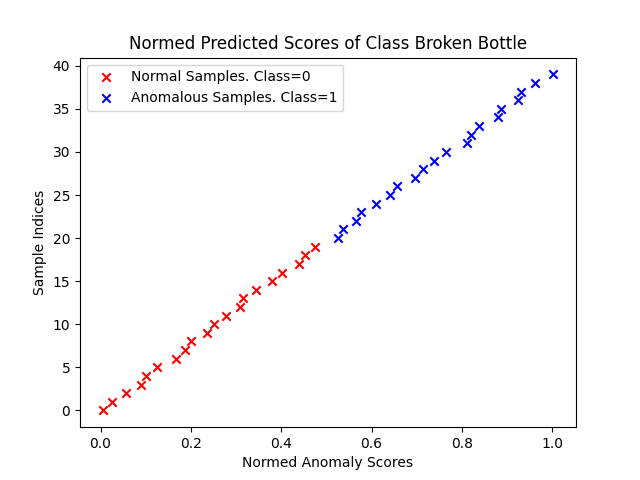
\includegraphics[width=\textwidth]{figures/anomaly_scores_sorted.png}
        \caption{Normed Predicted Anomaly Scores for 20 Images of the Broken Bottle Class and 20 Normal Images}
        \label{fig:scoresNormed}
    \end{subfigure}
    \hfill
    \begin{subfigure}[b]{0.4\textwidth}
        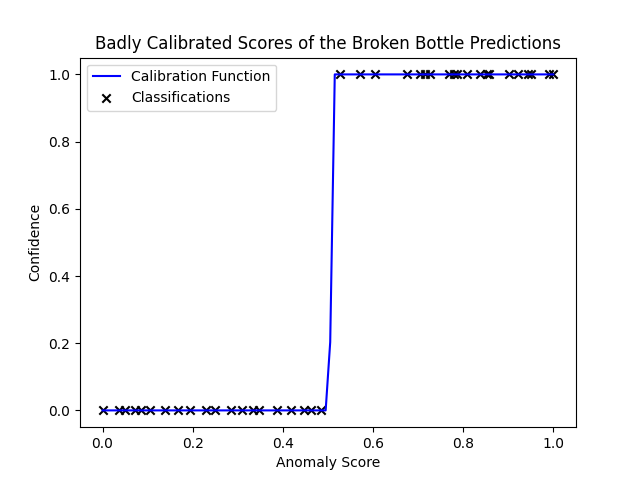
\includegraphics[width=\textwidth]{figures/anomaly_calibration_step.png}
        \caption{Applied Platt Scaling Calibration for the Normed Scores}
        \label{fig:platt}
    \end{subfigure}
    \caption{Sorted Normed Anomaly Scores for MVTecAD Class Broken Bottle and Applied Platt Scaling Calibration}
    \label{fig:badCal}
\end{figure}

Due to the high performance of some IAD algorithms it is possible that some categories 
of the datasets are fully correctly classified, which in example was the case for this. This would mean, that the optimal fitted sigmoid curve on the points 
is a step curve, yielding either 100 percent confidence or none at all. This of course does not seem well calibrated, especially not looking at the exemplary score distribution in figure \ref{fig:platt}, where it 
apprears that the predicted anomaly scores seem to be stretched pretty evenly over the interval. To overcome this problem 
we propose a generalized bounded sigmoid function with a varibale slope \cite{bounded_sigmoid} as seen in equation \ref{eq:boundedsigmoid}. This allows the user to calibrate the steepness of the slope to account for larger uncertainty 
towards the decision threshold.

\begin{equation}
    \label{eq:boundedsigmoid}
    \begin{split}
        s_{k, t}(x) = \frac{1}{1 + (x^{\frac{log(2)}{log(t)}} - 1)^{k}}
    \end{split}
\end{equation}

T denotes the point where the function has to pass through. This value is usually assigned the calculated threshold for the decision criterion of the classification task. K is a parameter 
that influences the growth of the curve along the axis. This value can either be chosen per hand or optimized in regards to uncertainty requirements. This means that if you generally want the 
ouputs to reflect a higher uncertainty towards the threshold it is resonable to chose a lower value for k and vice versa. Figures \ref{fig:sub1} and \ref{fig:sub2} demonstrates the effects of different values for k, as well 
as an exemplary well calibrated platt scaling variant of figure \ref{fig:sub3}, using the presented formula.

\begin{figure}[htbp]
    \centering
    \begin{subfigure}[b]{0.3\textwidth}
        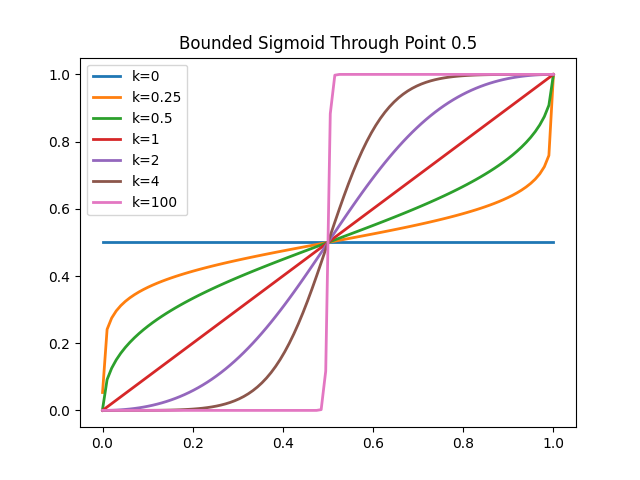
\includegraphics[width=\textwidth]{figures/soft_sigmoidt05.png}
        \caption{Function Values for t=0.5 and Various k-Values}
        \label{fig:sub1}
    \end{subfigure}
    \hfill
    \begin{subfigure}[b]{0.3\textwidth}
        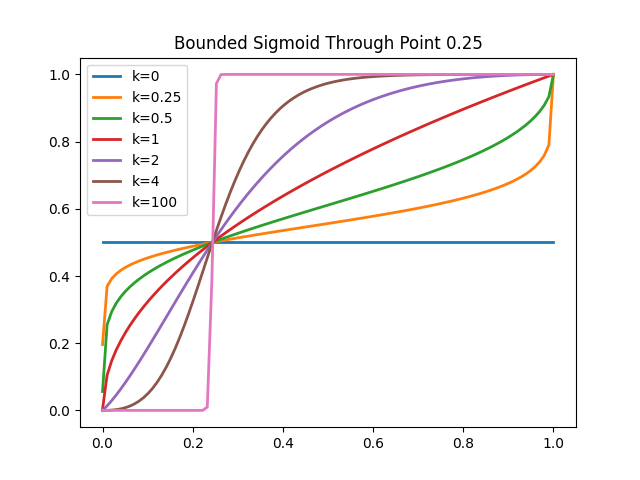
\includegraphics[width=\textwidth]{figures/soft_sigmoidt25.png}
        \caption{Function Values for t=0.25 and Various k-Values}
        \label{fig:sub2}
    \end{subfigure}
    \begin{subfigure}[b]{0.3\textwidth}
        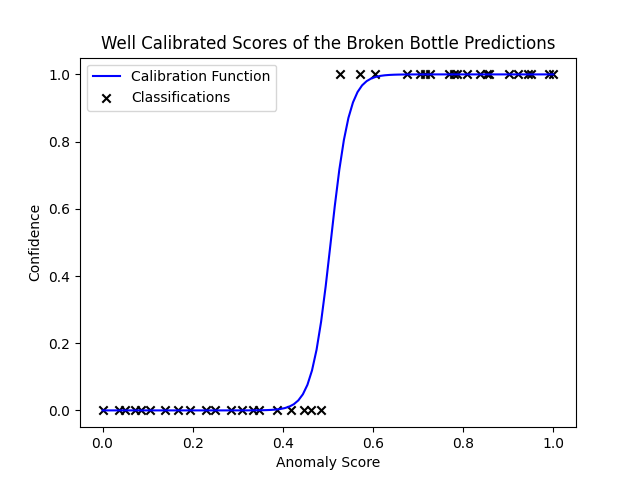
\includegraphics[width=\textwidth]{figures/anomaly_calibration_soft.png}
        \caption{Well Calibrated Scoring Function for Broken Bottle Class}
        \label{fig:sub3}
    \end{subfigure}
    \caption{Different Effects of Changing Parameters k and t and Exemplary Calibration for MVTecAD Class Broken Bottle}
    \label{fig:main}
\end{figure}

This caliration method is provided in the pipeline to produce an uncertainty metric. Yet in the light of the reported metrics of other IAD research the experiments and discussion will only 
review the same metrics, namely image and pixel AUROC and the PRO, or rather sPRO, score.








